\documentclass{article}%
\usepackage[T1]{fontenc}%
\usepackage[utf8]{inputenc}%
\usepackage{lmodern}%
\usepackage{textcomp}%
\usepackage{lastpage}%
\usepackage[head=40pt,margin=0.5in,bottom=0.6in]{geometry}%
\usepackage{graphicx}%
%
\title{\textbf{España planteará ante la UE cambiar sanciones por diálogo con Venezuela}}%
\author{El Nacional Web}%
\date{14/10/2018}%
%
\begin{document}%
\normalsize%
\maketitle%
\textbf{URL: }%
http://www.el{-}nacional.com/noticias/politica/espana{-}planteara{-}ante{-}cambiar{-}sanciones{-}por{-}dialogo{-}con{-}venezuela\_255700\newline%
%
\textbf{Periodico: }%
EN, %
ID: %
255700, %
Seccion: %
Política\newline%
%
\textbf{Palabras Claves: }%
España, Nicolás Maduro, Política, Europa\newline%
%
\textbf{Derecho: }%
CONTEXTO%
, Otros Derechos: %
NO\_TIENE%
, Sub Derechos: %
NO\_TIENE%
\newline%
%
\textbf{EP: }%
NO\newline%
\newline%
%
\textbf{\textit{La decisión será tomada este lunes durante el consejo de ministros de Asuntos Exteriores de la Unión Europea}}%
\newline%
\newline%
%
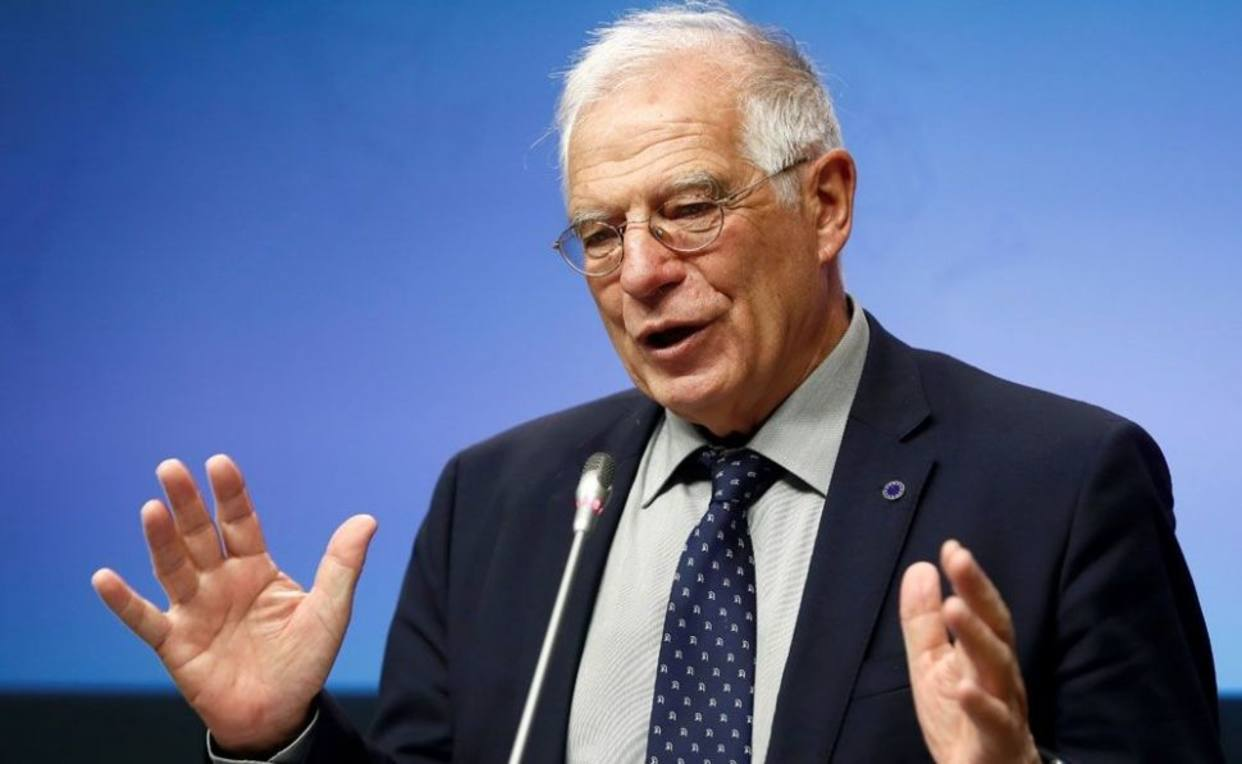
\includegraphics[width=300px]{107.jpg}%
\newline%
%
El ministro de Exteriores de España, Joseph Borrell, apelará por la defensa de la democracia y los derechos humanos de Venezuela;~sin embargo, apoyará el diálogo como una medida para que el país pueda salir de la crisis política y económica que atraviesa.%
\newline%
%
Con esta propuesta, dejaría~a un lado la posibilidad de implementar sanciones a los funcionarios venezolanos, lo que contradice las acciones adoptadas por el presidente de Estados Unidos, Donald Trump, reseñó~El País~de España.%
\newline%
%
Si se toma en cuenta la medida, España iría contra la estrategia implementada por el gobierno de Mariano Rajoy, que había impulsado un castigo diplomático por parte de la UE para el gobierno de Nicolás Maduro.%
\newline%
%
La decisión será tomada este lunes durante el consejo de ministros de Asuntos Exteriores de la Unión Europea. Los funcionarios se reunirán en un almuerzo para abordar el tema de Venezuela, por lo que existe la posibilidad de que no lleguen a un acuerdo determinante.%
\newline%
%
Lea más en~El País.%
\newline%
%
\end{document}